% !TeX root = ../../thesis.tex

A \ac{bn} with structure and parameters learned from the training dataset reached an average \ac{auroc} of 0.857. The results are in the table \ref{tab:result_auc}.



\begin{table}[htpb]
 \caption{Repeated Cross-Validation (10x2) Results: Column acronym with \ac{auroc} along with 95\% \ac{ci}. Acronym description is available in appendix \ref{appendix:data_dict}} \label{tab:result_auc} 

\renewcommand{\arraystretch}{1.2}
%\setlength{\tabcolsep}{8pt}
\centering
\begin{tabular} { p{1.5cm} p{1.5cm} p{3cm} p{1.5cm} p{1.5cm} l }
\hline
AP & 0.944 & [0.943, 0.945] & VNH & 0.894 & [0.893, 0.895] \\
AG & 0.797 & [0.778, 0.816] & TPEE & 0.816 & [0.815, 0.816] \\
EA & 0.969 & [0.968, 0.969] & AA & 0.751 & [0.743, 0.758] \\
CA & 0.958 & [0.958, 0.958] & GR & 0.931 & [0.93, 0.932] \\
IA & 0.638 & [0.637, 0.638] & V & 0.983 & [0.982, 0.983] \\
PI & 0.881 & [0.88, 0.881] & TP & 0.866 & [0.865, 0.868] \\
IMC & 0.881 & [0.881, 0.882] & VCS & 0.79 & [0.789, 0.791] \\
NRC & 0.75 & [0.75, 0.75] & ANP & 0.942 & [0.938, 0.946] \\
IGA & 0.968 & [0.968, 0.969] & GS & 0.514 & [0.507, 0.52] \\
SGP & 0.974 & [0.974, 0.974] & S & 0.896 & [0.896, 0.897] \\
VA & 0.974 & [0.974, 0.974] & VP & 0.771 & [0.77, 0.772] \\
TG & 0.728 & [0.726, 0.73] & TPNP & 0.952 & [0.951, 0.952] \\
\hline
 \multicolumn{6}{c}{\textbf{Average}  \textbf{0.857 [0.846, 0.868]}} \\

\hline
\end{tabular}
\end{table}


The network is as represented in figure \ref{fig:network}.
%TC:ignore
\begin{figure}[htbp]
\centering
\caption{Network learned}\label{fig:network} 
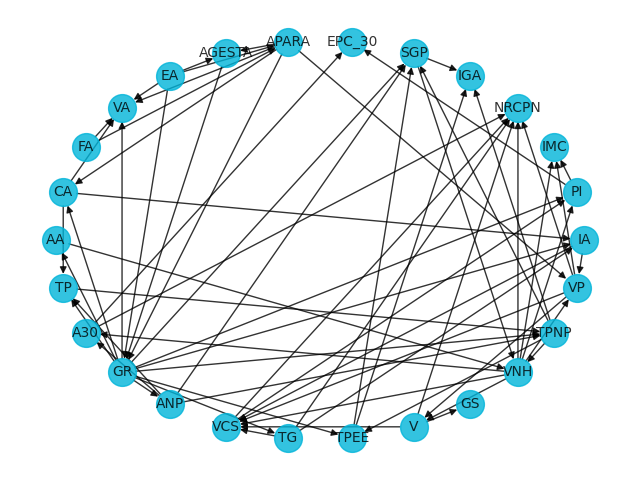
\includegraphics[scale=0.68]{figures/network.png}
\end{figure}
%TC:endignore

As for the rules created, they were conformance-based, like the format of dates, and conformance to the value set (i.e. Robson group, bishop scores, or delivery types). We also added plausibility rules, like expected values for BMI, weight, and gestational age. We also added plausibility for the relationship between columns, namely weight across different weeks of gestation. We have also added a relationship of greatness between ultrasound weights more than 5 weeks apart. 
The method of calculating the final score is stated in figure \ref{fig:wf}.


%TC:ignore
\begin{figure}[htbp]
    \centering
    \caption{Workflow for creating the final score and which elements are used to do so}\label{fig:wf} 
    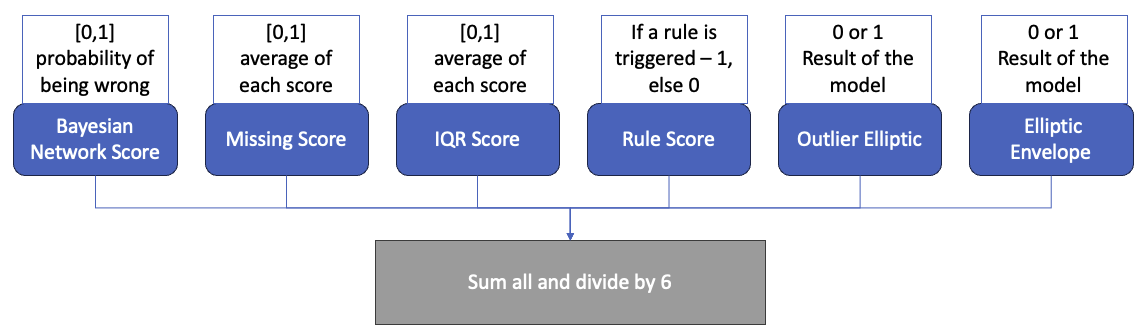
\includegraphics[scale=0.38]{figures/wf-update-dq.png}
    \end{figure}
    %TC:endignore


\subsection{Deployment \& Validation}
The purpose of this model is to serve as an \ac{api} for usage within a healthcare institution and act as a supplementary data quality assessment tool. Although a concrete, vendor-specific information model and health information system were initially used, our goal is to develop a more universal clinical decision support system. This system should be usable across all systems involved in birth and obstetrics departments. Therefore, we constructed it using the \ac{hl7} \ac{fhir} R5 version standard. This approach simplifies the process of API interaction. Rather than utilizing a proprietary model for the data, we based our decision on the use of \ac{fhir} resources: Bundle and Observation. These resources handle the request and response through a customized operation named "\$quality\_check". We intend to publish the profiles of these objects to streamline API access via standardized mechanisms and data models. The model then makes use of the customized operation and of several base resources to construct a \ac{fhir} message, which are: Bundle, MessageHeader, Observation, Device. Observation is where the information about the record is contained, Device contains information about the model, and MessageHeader is used to add information about the request. Finally, the Bundle is used to group all of these resources together. The current version of the profiles can be accessed here \cite{almeidaObstetricsClinicalDecision}.

For validation, we deployed the tool in docker format in a hospital to gather new data. We gathered 3231 new cases and returned a score for quality as exemplified in figure \ref{fig:scores}. Being that the score is from 0 to 1, the average score was 0.23 and \ac{iqr} was 0.03.
As for the clinicians' assessment, we got 4 answers. Figure \ref{fig:clinical_dq} shows the aggregated rankings of the clinicians per record and is ordered by the rank provided by the model.



%TC:ignore
\begin{figure}[htbp]
\centering
\caption{Model score for newly seen data}\label{fig:scores} 
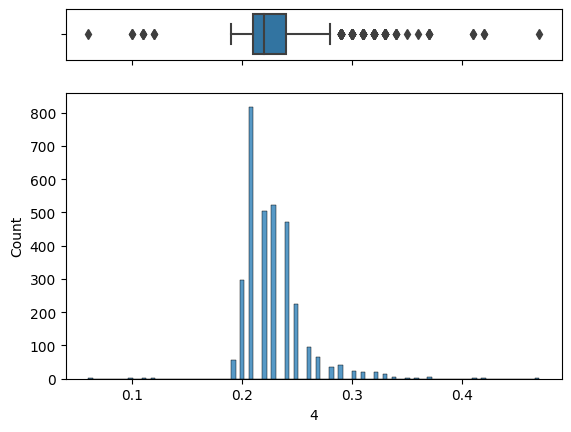
\includegraphics[scale=0.78]{figures/Scoring.png}
\end{figure}
%TC:endignore

%TC:ignore
\begin{figure}[htbp]
\centering
\caption{Comparison of clinical assessment of records with the model. Y is the clinicians' assessment, X is the ranking of the record per the model. Equal numbers on the X mean a tie per the model interpretation. Color is the record ID.}\label{fig:clinical_dq} 
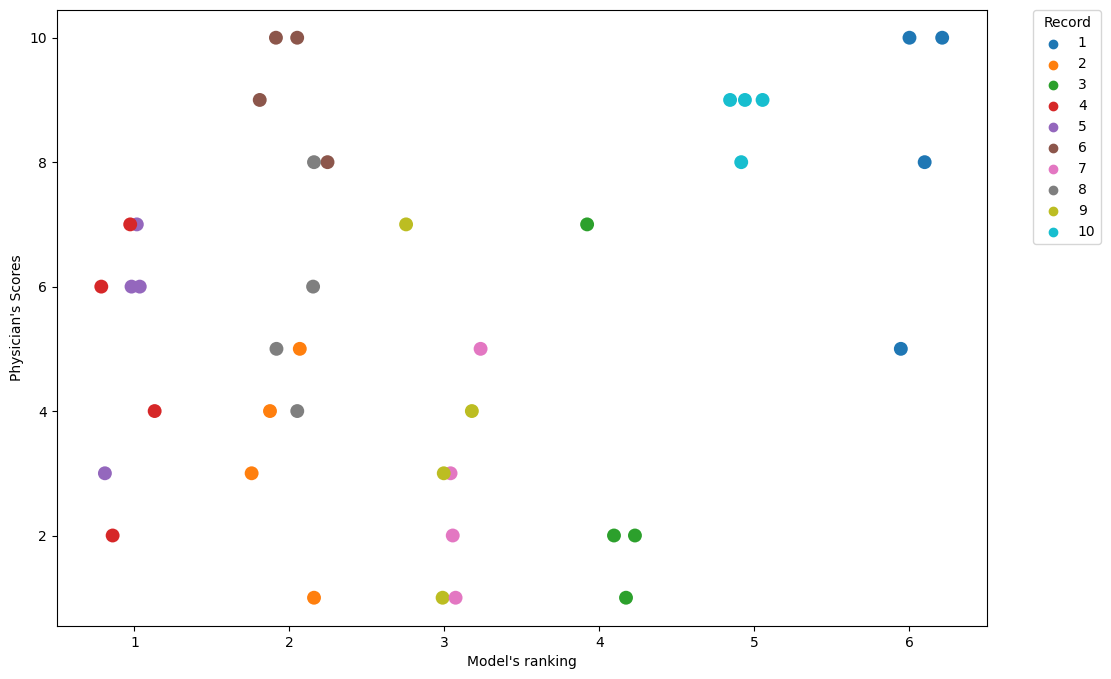
\includegraphics[scale=0.52]{figures/clinical_assessment_dataqual_scatter.png}
\end{figure}
%TC:endignore

The Average Spearman's Rank Correlation Coefficient was 0.04 and the Kendall's Tau was 0.0 with a \textit{P} value of 1. Defining the threshold for the model at 0.23 and the threshold for the physician at 8, we got an accuracy of 0.9, precision of 1, recall of 0.66 and f1-score at 0.8.
